

\section{Measures}

\subsection{Idle}
We define idle time to be the time where the driver might as well have turned off the engine. 
When a vehicle is decelerating with the clutch down the RPM of the engine will drop to idle, however, the driver may not turn of the engine of in this situation as he would lose power, stearing and break assistance. 
The avarage lowest RPM is 800-850 RPM. 
We therefore define idle state as when the speed of the vehicle is less than 10 km/h and the RPM of the engine is less than 900.

The percentage of idle time in each trip is show in Figure \ref{fig:kmlTrips}. 
The number of trips is on the y-axis and the percentage of idle time is the x-axis. 
It is clear that the majority of trips with low km/l have a high percentage of idle time. 
And the trips with high km/l have less idle time.

\begin{figure}[htb]
\centering
\includegraphics[width=0.5\textwidth]{../src/images/idle_percentageTrips.png}
\caption{Idle time all trips}
\label{fig:kmlTrips}
\end{figure}

\subsection{Cruise}

\cite{} establishes that driving at a constant speed is more fuel echonomic. 
From observing data with and without the driver using cruise control we find that the speed varies $\pm$ 1km/h. 
An experienced driver can drive at a constant speed without cruise control but the speed will generaly vary more. 
We define a vehicle as cruising if it in a 40 second period drive with a constant speed $\pm$ 1km/h.

Figure~\ref{fig:cruiseTrips} shows how often the trips cruise. 
Almost all trips never cruise, and all trips classified as having a low km/l never cruise.

\begin{figure}
\centering
\includegraphics[width=0.5\textwidth]{../src/images/cruise_percentageTrips.png}
\caption{Cruise all trips}
\label{fig:cruiseTrips}
\end{figure}

\subsection{acckm}

Acckm capture the sum of accelerration a vehicle perform on a trip. \cite{} establishes that accelerrating consume extra fuel. A trip with a low accelerration should use less fuel. To normalise acckm we divide it by the lenght of the trip. Acckm is caculated in Algorithm \ref{alg.acckm}. A buffer (dotted line) as shown in Figure \ref{fig:acckm} is implemented to prevent small variaction in speed (solid line) to effect the acckm

\begin{algorithm}
\caption{$acckm$}\label{alg.acckm}
\begin{algorithmic}[1]
\State $temp = 0$
\State $counter = 0$
\State $buffer = 5$
\While{$i < n$}
\If{$v_i - v_{i-1} > buffer$}
	\State $counter += (v_i - v_{i-1}) - buffer$
	\State $temp = v_i - buffer$
\ElsIf{$v_{i-1} - v_i > buffer$}
	\State $temp = v_i + buffer$
\EndIf
\State $i+=1$
\EndWhile
\State \Return $ counter / trip_{length}$

\end{algorithmic}
\end{algorithm}

Figure \ref{fig:acckm} show the number of trips on the y axis having a acckm show on the x axis. Trips with a high km/l are mostly clustered with a low acckm and vice versa. 

\begin{figure}[htb]
\centering
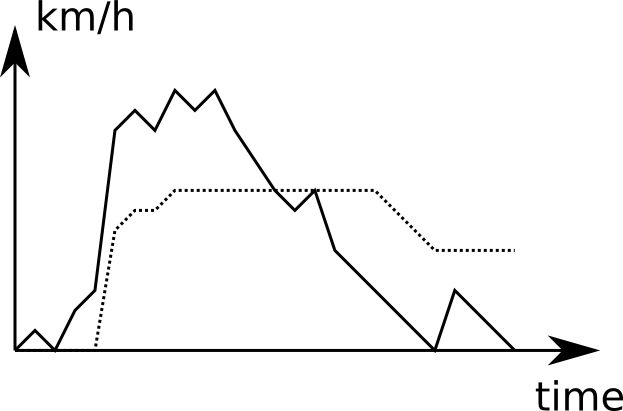
\includegraphics[width=0.4\textwidth]{../images/acckm.png}
\caption{Acckm}
\label{fig:acckm}
\end{figure}

\begin{figure}
\centering
\includegraphics[width=0.5\textwidth]{../src/images/acckmTrips.png}
\caption{Acceleration km all trips}
\label{fig:acckmTrips}
\end{figure}

\subsection{Stop and go}

Stop and go represents the number of times a vehicle decelerates below 10 km/h and accelerates up above 15 km/h, normalised over the lenght of the trip.
%TODO: Experiments

Figure~\ref{fig:stopngoTrips} shows the number of trips in for each three classes as a function over how many stops they make in the trip.
We clearly see that the trips classified as having a high km/l have less stops than those in the medium class.

\begin{figure}
\centering
\includegraphics[width=0.5\textwidth]{../src/images/stopngoTrips.png}
\caption{Number of stop and go's all trips}
\label{fig:stopngoTrips}
\end{figure}
